\documentclass[a4paper]{article}

%% Language and font encodings
\usepackage[english]{babel}
\usepackage[utf8x]{inputenc}
\usepackage[T1]{fontenc}

%% Sets page size and margins
\usepackage[a4paper,top=3cm,bottom=2cm,left=3cm,right=3cm,marginparwidth=1.75cm]{geometry}

%% Useful packages
\usepackage{amsmath}
\usepackage{amssymb}
\usepackage{breqn}
\usepackage{graphicx}
\usepackage[colorinlistoftodos]{todonotes}
\usepackage[colorlinks=true, allcolors=blue]{hyperref}
%\usepackage[colorlinks=true, allcolors=black]{hyperref}
\usepackage[linesnumbered,ruled]{algorithm2e}

%\title{Group Recommendation on Yelp Dataset with Markov Chain Monte Carlo and Collaborative Filtering}
\title{Group Recommendation based on Collaborative Filtering and Markov Chains}

\author{ {\rm Nicholas Gao, Evin Pinar Örnek, Jan Sültemeyer} \\ \textit{Technical University of Munich}}

\date{}

\begin{document}
\maketitle

\begin{abstract}
In this work, we present an end-to-end group recommendation pipeline, based on predicting restaurant ratings for individual users via collaborative filtering, followed by aggregating the individual restaurant rankings for a group.
For collaborative filtering, graph-regularized joint matrix factorization is employed, and the rank aggregation is solved via Markov Chain Monte Carlo simulations. Our whole system is trained on a dataset provided by Yelp as part of a public challenge. We have tested the recommendation pipeline from end to end as well as the individual components. Whereas our evaluation results based on Kendall-Tau distances are promising, further real world experiments should be conducted.
\end{abstract}

\section{Introduction}
This work describes a group recommendation algorithm developed with a dataset of restaurant ratings provided by Yelp\footnote{\href{https://www.yelp.com/dataset/challenge}{yelp.com/dataset/challenge}}.
It tackles the problem of finding a suitable restaurant for a group of people which everyone can enjoy, and solves it in a two-step process. First, we predict how each user in the group would rate a list of possible restaurants they have not necessarily been to before. In a second step, we use these predicted ratings to find the best suited restaurants for our group. For the rating prediction we use collaborative filtering based matrix factorization, which is a standard approach for building recommendation systems \cite{Dheeraj15}. Finding the best restaurants is then done by solving a rank aggregation problem \cite{Dwork03}, where we first order the restaurants from best to worst for each user, and then try to find an optimal aggregated order for the group. The problem of finding an optimal order of recommendations for a group is not well defined since soft social parameters often play a big role during the decision making of a group \cite{mccarthy2006group,katarya2017systematic,jameson2004more}.

This work is structured as follows: in Section \ref{sec:MatrixFactorization} a short introduction to different Matrix Factorization algorithms is given, followed by a description of group recommendation algorithms in Section \ref{sec:GroupRecommendation}. Section \ref{sec:Results} contains exemplary results, as well as an evaluation of our model, and Section \ref{sec:Conclusion} gives a short conclusion.

The code for this project is freely available on \href{https://github.com/n-gao/yelp-group-recommender}{GitHub}.


\section{Rating Prediction by Matrix Factorization}\label{sec:MatrixFactorization}

\subsection{Single Matrix Factorization}
We predict how a user would rate an unseen restaurant by factorizing a matrix $\mathbf{R} \in \mathbb{R}^{n \times m}$ containing star ratings from 1 to 5 stars is given by $n$ users to $m$ restaurants. This matrix is very sparse as we have $n = 1.3 \cdot 10^6$ and $m = 1.7 \cdot 10^5$.
We try to find two matrices $\mathbf{U} \in \mathbb{R}^{n \times k}$ and  $\mathbf{V} \in \mathbb{R}^{m \times k}$ that give a low dimensional, e.g. $k=128$ approximation to the rating matrix $\mathbf{R} \approx\mathbf{U}\mathbf{V}^T$  by minimizing the following sum over the nonzero entries of $\mathbf{R}$, where $\mathbf{u}_i, \mathbf{v}_j$ are the row vectors of $\mathbf{U}, \mathbf{V}$
\begin{equation}
\underset{\mathbf{U}, \mathbf{V}}{\operatorname{argmin}} \left(
\sum_{(i,j) \in \mathbf{R}} \left(\mathbf{R}_{ij} - \mathbf{u}_i \mathbf{v}_j^T\right)^2 \right).
\end{equation}

Each row of the matrix $\mathbf{U}$ contains a low dimensional embedding of a user, hopefully describing his taste in restaurants, and $\mathbf{V}$ is made up of low dimensional representations of restaurants. We can predict the rating that user $i$ will give to restaurant $j$ by computing $\mathbf{u}_i \mathbf{v}_j^T$.

\subsection{Joint Factorization}\label{subsec:joint}

Inspired by the work of Gupta et al. \cite{gupta2015collective} we performed a joint factorization of multiple matrices. However we decided to use different matrices and evaluated the performance gains of the individual matrices.

To improve the rating prediction we can add more information to our factorization model and jointly factorize four matrices, which are 
the rating matrix $\mathbf{R}$,
a friendship matrix $\mathbf{F} \in \mathbb{R}^{n \times n}$ that has a $1$ on position $(i,j)$ if users $i$ and $j$ are friends,
a restaurant relation matrix $\mathbf{A} \in \mathbb{R}^{m \times m}$ that introduces connections between restaurants if they have been rated in a similar way by some users,
and an attribute matrix $\mathbf{B} \in \mathbb{R}^{m \times d}$ that indicates for each restaurant which of $d$ attributes it possesses. For the construction of $\mathbf{A}$, we introduce two hyperparameters to control its density, a maximal distance between two reviews and a minimal number of users. The factorization model is then given as
\begin{align}
{\begin{pmatrix}
  &    & \\
  & \mathbf{R} &\\
  &     &
\end{pmatrix}
\mkern-10mu}_{m \times n} &\approx
{\begin{pmatrix}
  &    & \\
  & \mathbf{V} &\\
  &     &
\end{pmatrix}
\mkern-10mu}_{m \times k}
{\begin{pmatrix}
  &    & \\
  & \mathbf{U}^T &\\
  &     &
\end{pmatrix}\mkern-10mu}_{k \times n} \\
{\begin{pmatrix}
  &    & \\
  & \mathbf{F} &\\
  &     &
\end{pmatrix}
\mkern-10mu}_{n \times n} &\approx
{\begin{pmatrix}
  &    & \\
  & \mathbf{U} &\\
  &     &
\end{pmatrix}
\mkern-10mu}_{n \times k}
{\begin{pmatrix}
  &    & \\
  & \mathbf{U}^T &\\
  &     &
\end{pmatrix}\mkern-10mu}_{k \times n} \\
{\begin{pmatrix}
  &    & \\
  & \mathbf{A} &\\
  &     &
\end{pmatrix}
\mkern-10mu}_{m \times m} &\approx
{\begin{pmatrix}
  &    & \\
  & \mathbf{V} &\\
  &     &
\end{pmatrix}
\mkern-10mu}_{m \times k}
{\begin{pmatrix}
  &    & \\
  & \mathbf{V}^T &\\
  &     &
\end{pmatrix}\mkern-10mu}_{k \times m} \\
{\begin{pmatrix}
  &    & \\
  & \mathbf{B} &\\
  &     &
\end{pmatrix}
\mkern-10mu}_{m \times d} &\approx
{\begin{pmatrix}
  &    & \\
  & \mathbf{V} &\\
  &     &
\end{pmatrix}
\mkern-10mu}_{m \times k}
{\begin{pmatrix}
  &    & \\
  & \mathbf{W} &\\
  &     &
\end{pmatrix}\mkern-10mu}_{k \times d}  .
\end{align}

\subsection{Graph-Based Regularization}
Based on the results of Cai et al.\cite{cai2011graph} and Chakraborty et al.\cite{chakraborty2015nonnegative} which presented graph-based regularization to improve the factorization for collaborative filtering, this joint matrix factorization model can be further improved by adding graph-based regularization constraints to the optimization problem. The friendship and business relation matrices $\mathbf{F}$ and $\mathbf{B}$ can be interpreted as adjacency matrices of two graphs, one describing the friendships between users and the other one the connections between similar restaurants.

We construct a cost function that adds a penalty if the low dimensional representation of two friends -- given as rows of $\mathbf{U}$ -- are far apart
\begin{equation}
\underset{\mathbf{U}}{\operatorname{argmin}} \left(\sum_{(i,j) \in \mathbf{F}}||\mathbf{u}_i - \mathbf{u}_j||_2^2 \right).
\end{equation}
For connected restaurants -- rows of $\mathbf{V}$ -- we add a similar term. 

\subsection{Word Matrices}
So far we only used the one to five star ratings that users gave to restaurants. However, the dataset also includes short review texts for each rating. This information can also help to improve our factorization model. We construct two more matrices $\mathbf{P} \in \mathbb{R}^{n \times c}$ and $\mathbf{S} \in \mathbb{R}^{m \times c}$ that indicate which words are contained in a review belonging to a user or to a restaurant, respectively. Here, $c$ is the number of all possible words and the matrix $\mathbf{S}$ has a $1$ at position $(i,j)$ if user $i$ used the word $j$ in one of his reviews. They are then factorized together with the matrices described in \ref{subsec:joint}

\begin{align}
{\begin{pmatrix}
  &    & \\
  & \mathbf{P} &\\
  &     &
\end{pmatrix}
\mkern-10mu}_{n \times c} &\approx
{\begin{pmatrix}
  &    & \\
  & \mathbf{U} &\\
  &     &
\end{pmatrix}
\mkern-10mu}_{n \times k}
{\begin{pmatrix}
  &    & \\
  & \mathbf{Z}^T &\\
  &     &
\end{pmatrix}\mkern-10mu}_{k \times c}  \\
{\begin{pmatrix}
  &    & \\
  & \mathbf{S} &\\
  &     &
\end{pmatrix}
\mkern-10mu}_{m \times c} &\approx
{\begin{pmatrix}
  &    & \\
  & \mathbf{V} &\\
  &     &
\end{pmatrix}
\mkern-10mu}_{m \times k}
{\begin{pmatrix}
  &    & \\
  & \mathbf{Z}^T &\\
  &     &
\end{pmatrix}\mkern-10mu}_{k \times c}
\end{align}

In our experiments, we also built these matrices such that the entries are normalized word frequencies and compared with the binary matrices. The binary relations worked better and we chose to apply those in our evaluations.

\subsection{Cost Function and Optimization}
The complete cost function we want to minimize is given as 
\begin{dmath}
\underset{\mathbf{U}, \mathbf{V}, \mathbf{W}, \mathbf{Z}}{\operatorname{argmin}} \left(
\sum_{(i,j) \in \mathbf{R}} \left(R_{i,j}-\mathbf{v}_i\mathbf{u}_j^T \right)^2 +
\sum_{(i,j) \in \mathbf{F}} \left(F_{i,j}-\mathbf{u}_i\mathbf{u}_j^T \right)^2 +
\sum_{(i,j) \in \mathbf{A}} \left(A_{i,j}-\mathbf{v}_i\mathbf{v}_j^T \right)^2 +
\sum_{(i,j) \in \mathbf{B}} \left(B_{i,j}-\mathbf{v}_i\mathbf{w}_j^T \right)^2 +
\sum_{(i,j) \in \mathbf{P}} \left(P_{i,j}-\mathbf{u}_i\mathbf{z}_j^T \right)^2 +
\sum_{(i,j) \in \mathbf{S}} \left(P_{i,j}-\mathbf{v}_i\mathbf{z}_j^T \right)^2 +
\lambda \left(||\mathbf{U}||_F^2 + ||\mathbf{V}||_F^2 + ||\mathbf{W}||_F^2 + ||\mathbf{Z}||_F^2 \right) +
\gamma \left(\sum_{(i,j) \in \mathbf{F}}||\mathbf{u}_i - \mathbf{u}_j||_2^2 +
\sum_{(i,j) \in \mathbf{A}}||\mathbf{v}_i - \mathbf{v}_j||_2^2 \right)
\right),
\end{dmath}
where the first six terms are describing the reconstruction error of the factorization model. An $\mathcal{L}^2$-regularization term is introduced for each matrix and weighted by $\lambda$ -- this helps keeping the values small. The graph-based regularization terms are weighted by the parameter $\gamma$.

The cost function can be minimized via alternating optimization, where we initialize all matrices with random values and iteratively update one of them while keeping the other matrices fixed. For each matrix we can update all rows independently. For one row $\mathbf{u}_i$ of the user matrix $\mathbf{U}$ -- i.e. the low dimensional embedding of one user -- we solve a least squares minimization problem where we stack the contributions of each term including $\mathbf{u}_i$ into one matrix
\begin{equation}
\underset{\mathbf{u}_i}{\operatorname{argmin}} \left(
\left| \left|
\begin{pmatrix}
  \mathbf{V}_i\\
  \mathbf{U}_i\\
  \mathbf{Z}_i \\
  \gamma \mathbf{I}
\end{pmatrix}
\mathbf{u}_i^T - 
\begin{pmatrix}
  \mathbf{r}_i \\
  \mathbf{f}_i \\
  \mathbf{p}_i \\
  \mathbf{u}_{avg}
\end{pmatrix}
\right| \right|_2^2
+ \lambda ||\mathbf{u}_i||_2^2 \right),
\end{equation}
where $\mathbf{V}_i$ is a matrix that includes all rows $\mathbf{v}_j$ -- i.e. business embeddings -- for which there is an entry in the rating matrix $R_{i,j}$. These ratings make up the vector $\mathbf{r}_i$. The matrices and vectors $\mathbf{U}_i$, $\mathbf{Z}_i$, $\mathbf{f}_i$, $\mathbf{p}_i$  are derived analogously. The terms $\gamma \mathbf{I}$ -- the scaled identity matrix -- and $\mathbf{u}_{avg}$ introduce the friendship graph-based regularization term. The vector $\mathbf{u}_{avg}$ is the average embedding vector of all the friends of user $i$. Minimizing the distance between $\mathbf{u}_i$ and $\mathbf{u}_{avg}$ is equivalent to minimizing the distances between $\mathbf{u}_i$ and all his friends individually. This least squares problem can be solved by using a linear solver for the normal equations
\begin{equation}
\left(
\begin{pmatrix}
  \mathbf{V}_i &
  \mathbf{U}_i &
  \mathbf{Z}_i &
  \gamma \mathbf{I}
\end{pmatrix}^T
\begin{pmatrix}
  \mathbf{V}_i\\
  \mathbf{U}_i\\
  \mathbf{Z}_i \\
  \gamma \mathbf{I}
\end{pmatrix}
+ \lambda \mathbf{I} \right)
\mathbf{u}_i^T
= 
\begin{pmatrix}
  \mathbf{V}_i &
  \mathbf{U}_i &
  \mathbf{Z}_i &
  \gamma \mathbf{I}
\end{pmatrix}^T
\begin{pmatrix}
  \mathbf{r}_i \\
  \mathbf{f}_i \\
  \mathbf{p}_i \\
  \mathbf{u}_{avg}
\end{pmatrix}.
\end{equation}
This $k$ dimensional linear system is solved for each row $\mathbf{u}_i$ and similar systems for the rows of $\mathbf{V}, \mathbf{W}$ and $\mathbf{Z}$.


\section{Group Recommendation}\label{sec:GroupRecommendation}

\subsection{Markov Chain Monte Carlo Aggregation Method}

Finding a best option among some items for a group is generally called the "consensus problem". It initially occurred on political decision systems in early times. The problem of "choosing the best representative among several candidates" lead to the discipline of social choice theory, which deals with the group decision making process and tries to choose the best option for all group members. There are several strategies to combine and aggregate users' decisions. The traditional approaches are classified as majority based, consensus based, and borderline methods\cite{Masthoff11}. Majority based algorithms focus on popularities of candidates, examples are Borda count, Copeland and Plurality voting strategies. Consensus algorithms, on the other hand, consider individual's preferences in a more democratic way, such as by averaging or multiplying them. And lastly, Borderline methods limit the results by constraints, either filtering out choices that would lead to miserable individuals, or assuming a single most important individual. 

These social choice algorithms  are used in computer science for solving problems involving decisions among several preference listings. Examples are aggregating search results coming from different search engines or deciding on recommendation items for a group of users. Among the social choice aggregation methods, Borda Count and Copeland strategies show promising results in different cases. However, a recent study based on a randomization strategy proved to work better than these traditional approaches \cite{Dwork03}. Hence, we apply this Markov Chain based aggregation method on our model. 

As an optimization metric, we choose Kendall-Tau distance which counts the number of pairwise differences between given lists. In our case, we have $a$ users in a group, and collaborative filtering which gives us $a$ lists of restaurants ordered by predicted rankings. The goal is to find an aggregated list of restaurants, which represents these $a$ lists in the best possible way, and minimizes the Kendall-Tau metric. In other words, given $a$ permutations $\tau_i$, we try to find a permutation $\tau$ which minimizes the Kendall-tau-distance between every $\tau_i$ and $\tau$. Our Markov Chain algorithm solves this optimization goal iteratively. The current state -- in our case a restaurant -- is denoted as $P$. We then choose $Q$ uniformly from all possible states and go to Q if $\tau_i(Q)<\tau_i(P)$ for the majority of users, otherwise we stay in $P$. Here,$\tau_i(Q)$ is the position of restaurant $Q$ in the preference list of user $i$, $\tau_i$. This way we could build a transition Matrix describing a Markov Chain.

Since this transition matrix is impractical to explicitly compute due to the high number of businesses, we use Monte Carlo simulation to approximate this Markov Chain. To get the best $m$ items, we use the following algorithm:

\begin{algorithm}[h]
\caption{Markov Chain Algorithm}\label{alg:euclid}
MC = MarkovChain\;
items = $\emptyset$\;
\While {len(items) < m} {
	$new\_items = monte\_carlo\_get\_next(MC)$\; 
    $MC.remove\_items(new\_items)$\;
    $items = items \cup new\_items$\;
}
\end{algorithm}

Here, in order to speed up the computation, we remove some of the highest ranked items -- which would be dead ends -- before running the Monte Carlo simulation and add them to our results without running in simulation. These items are basically the ones that proved to be the best ones and they are collected as results.

\subsection{System Pipeline}

In order to efficiently provide a group recommendation for Yelp users from a large dataset of possibilities, we applied some optimization steps to speed up the overall process. Our pipeline can be described as: 
\begin{enumerate}
\item 
\begin{enumerate}
\item Collaborative filtering, compute $\mathbf{U}$ and $\mathbf{V}$
\item Overwrite predicted ratings with real ratings where possible 
\end{enumerate}
\item
\begin{enumerate}
\item Filter possible restaurants, i.e. choose city and discard e.g. $\%50$ of the least rated items
\item Predict rating for these restaurants for each group member, project them to $[1,5]$
\item Order each user's individual list according to rankings
\item Markov Chain Monte Carlo simulation to find the best recommendation.
\end{enumerate}
\end{enumerate}

Here, the first steps -- i.e. collaborative filtering --  need to be computed once and updated only when new data becomes available, whereas the second steps are executed for each recommendation task.

\section{Results}\label{sec:Results}

Since our group recommender system consists of two parts, the collaborative filtering and the rank aggregation, first we test the accuracy of these two models individually. Then, we evaluate our end-to-end multi stage recommender pipeline. 

\subsection{Matrix Factorizations}
To test the accuracy of different matrix factorization methods, we split our data the  the train set $80\%$, validation set $10\%$ and test set $10\%$. To find the best model, we compare different methods described in section \ref{sec:MatrixFactorization} and three different hyperparameters -- $\lambda$ - L2 regularization weight, $\gamma$ - graph regularization weight, $k$ - Latent space dimension -- and perform an exhaustive search. In a first run, we compare the validation loss for $540$ different set-ups with models factorizing the four matrices $\mathbf{R}, \mathbf{F}, \mathbf{A}$, and  $\mathbf{B}$, the two matrices $\mathbf{R}$ and $\mathbf{B}$, or only $\mathbf{R}$. The results  for the best $10$ set-ups are shown in Table \ref{fig:mf_result_1}.
\begin{table}[h]
\centering
\begin{tabular}{| l | l | l | l | l |}
\hline
Used Matrices & k & $\lambda$ & $\gamma$ & Validation Loss \\ \hline
$\mathbf{R}, \mathbf{F}, \mathbf{A}, \mathbf{B}$ & 256 & 2 & 1 & 1524.1 \\ \hline
$\mathbf{R}, \mathbf{F}, \mathbf{A}, \mathbf{B}$ & 32 & 2 & 2 & 1525.8 \\ \hline
$\mathbf{R}, \mathbf{F}, \mathbf{A}, \mathbf{B}$ & 32 & 0.5 & 2 & 1526.0 \\ \hline
$\mathbf{R}, \mathbf{F}, \mathbf{A}, \mathbf{B}$ & 128 & 1 & 2 & 1527.3 \\ \hline
$\mathbf{R}, \mathbf{F}, \mathbf{A}, \mathbf{B}$ & 64 & 1 & 2 & 1527.7 \\ \hline
$\mathbf{R}, \mathbf{B}$ & 512 & 2 & 1 & 1528.7 \\ \hline
$\mathbf{R}, \mathbf{F}, \mathbf{A}, \mathbf{B}$ & 32 & 2 & 1 & 1528.8 \\ \hline
$\mathbf{R}, \mathbf{B}$ & 512 & 1 & 2 & 1533.8 \\ \hline
$\mathbf{R}, \mathbf{F}, \mathbf{A}, \mathbf{B}$ & 128 & 2 & 2 & 1535.2 \\
\hline
\end{tabular}
\caption{\label{fig:mf_result_1}The results of factorizations for 4,2, and 1 input matrices with graph regularization. Different sets of latent dimensions $k$, $\mathcal{L}^2$ regularization coefficient $\lambda$, and graph regularization coefficient $\gamma$ are tested and compared w.r.t. the loss on the validation set. As can be seen from the sorted order of the results, using four matrices and $k=256$ worked best among all.}
\end{table}

In a second step, we added the word Matrices $\mathbf{P}$ and $\mathbf{S}$ and compared the models in a similar fashion, as can be seen in Table \ref{fig:mf_result}

\begin{table}[h]
\centering
\begin{tabular}{| l | l | l | l | l |}
\hline
Used Matrices & k & $\lambda$ & $\gamma$ & Optimization Loss \\ \hline
$\mathbf{R}, \mathbf{F}, \mathbf{A}, \mathbf{B}$  & 256 & 2 & 1 & 1524.1 \\ \hline
$\mathbf{R}, \mathbf{F}, \mathbf{A}, \mathbf{B}$ & 256 & 1 & 2 & 1524.2 \\ \hline
$\mathbf{R}, \mathbf{F}, \mathbf{A}, \mathbf{B}, \mathbf{P}, \mathbf{S}$ & 64 & 1 & 2 & 1526.2 \\ \hline
$\mathbf{R}, \mathbf{F}, \mathbf{A}, \mathbf{B}, \mathbf{P}, \mathbf{S}$ & 32 & 3 & 0.5 & 1526.7 \\ \hline
$\mathbf{R}, \mathbf{F}, \mathbf{A}, \mathbf{B}$  & 64 & 2 & 2 & 1526.9 \\ \hline
$\mathbf{R}, \mathbf{F}, \mathbf{A}, \mathbf{B}$  & 128 & 0.5 & 2 & 1526.9 \\ \hline
$\mathbf{R}, \mathbf{F}, \mathbf{A}, \mathbf{B}, \mathbf{P}, \mathbf{S}$ & 32 & 1 & 1 & 1527.0 \\ \hline
$\mathbf{R}, \mathbf{F}, \mathbf{A}, \mathbf{B}$  & 64 & 1 & 2 & 1527.2 \\ \hline
$\mathbf{R}, \mathbf{F}, \mathbf{A}, \mathbf{B}, \mathbf{P}, \mathbf{S}$ & 64 & 3 & 0.5 & 1528.1 \\
\hline
\end{tabular}
\caption{\label{fig:mf_result}The results of our second hyperparameter search. Using the word matrices $\mathbf{P}$ and $\mathbf{S}$ behaved contrary to our expectations and  did not improve the results.}
\end{table}

The results indicate that strong regularization terms are favored and the addition of the word matrices have no measurable effect on our performance, so we decided to discard them.

After this, we performed a last hyperparameter search to determine the density of our restaurant graph matrix $\mathbf{A}$. The best result is achieved by defining two restaurants to be similar only when they were rated with the same rating by at least two users. This indicates that a less dense matrix with only edges between same review scores contains the most relevant information.

With the best model, we achieve a Root-Mean-Squared-Error (RMSE) of 1.128 on the test set.
As a baseline for comparison we use the user mean as prediction for each restaurant, which gives a RMSE of 1.169. Our model improves this by 3.5\%.

While this seems like a small difference, we investigated this phenomenon further and analyzed the  results of Ma, et al. \cite{Ma08} -- they use four different matrix factorization algorithm. We compared thir results with the prediction of the user mean and noticed that three out of these four methods actually performed worse than the mean prediction. Predicting the mean gave us for an 80\% training-test split a mean absolute error of 0.97. The presented methods, reported errors of 1.0371, 1.0277, 0.9998 and 0.9321.

%\begin{figure}[h]
%\centering
%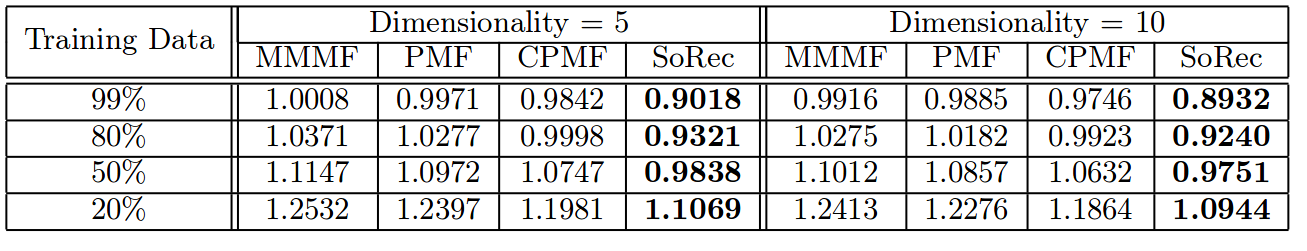
\includegraphics[width=0.9\textwidth]{table_MF.png}
%\caption{\label{fig:MF_table}This frog was uploaded via the project menu.}
%\end{figure}

\subsection{Rank Aggregation Methods}

In order to test our Markov Chain Aggregation algorithm, we chose a group of $N=10$ users and compared our results with other aggregation algorithms: Borda Count and rank averaging. The results can be seen in figure \ref{fig:kendalltau}. 

\begin{figure}[h]
\centering
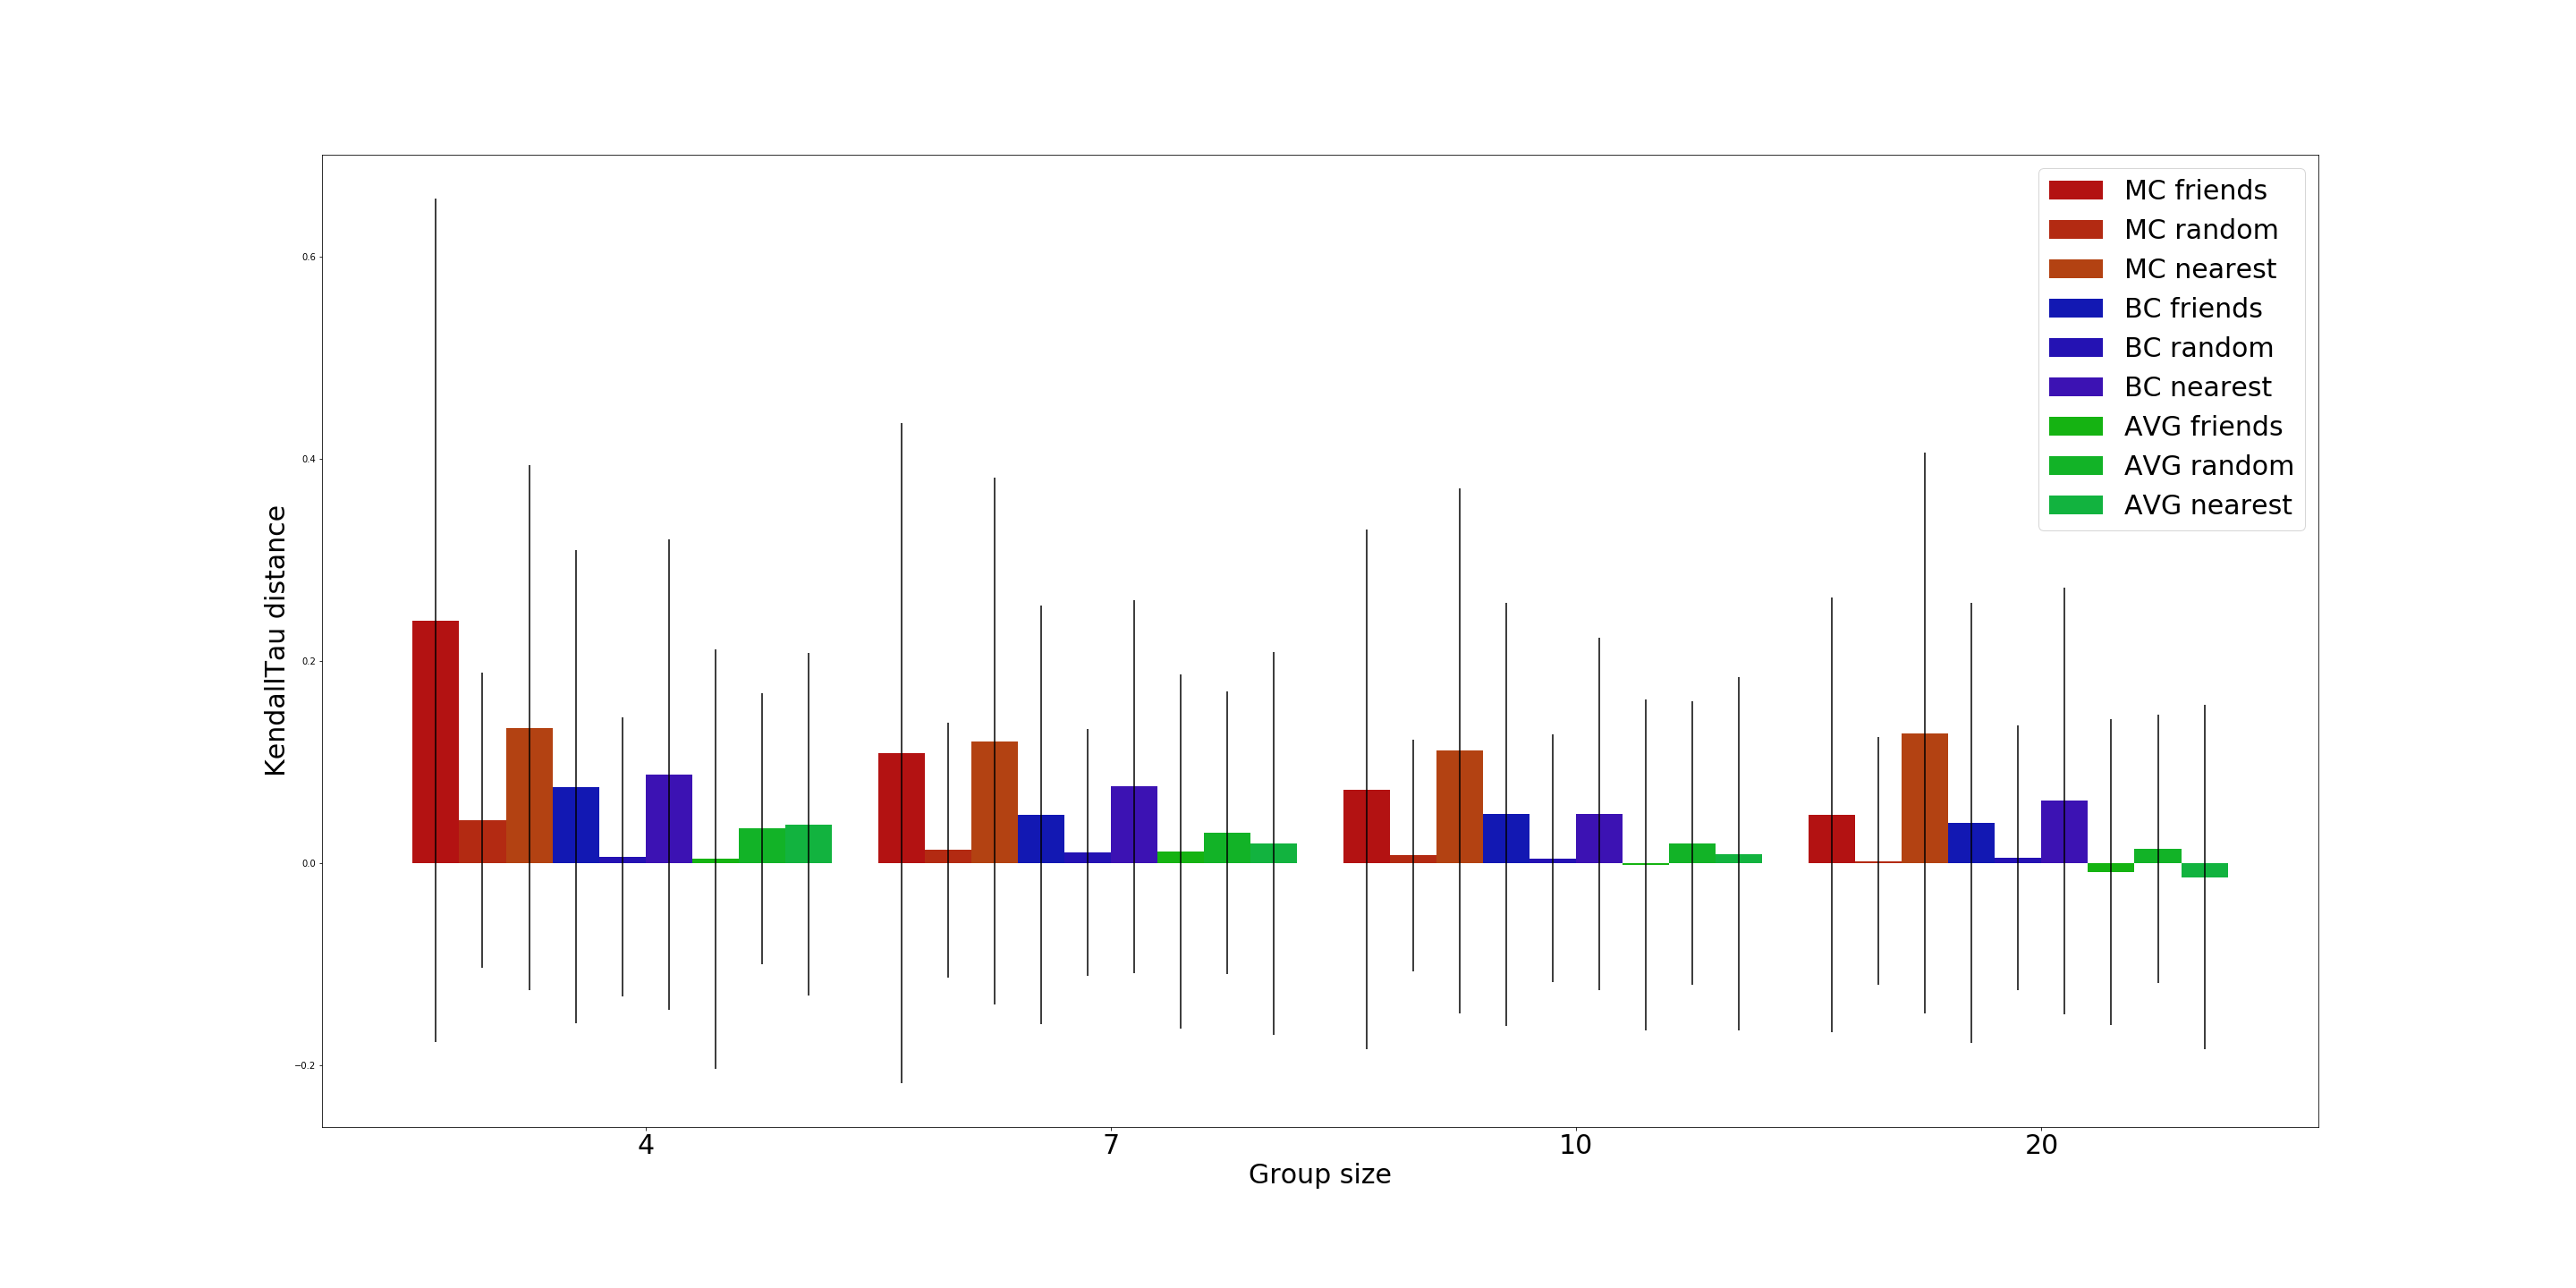
\includegraphics[width=0.9\textwidth]{kendalltau.png}
\caption{\label{fig:kendalltau}The Kendall-Tau distance results of Markov Chain, Borda Count and Average Rank Aggregation methods are illustrated. A positive Kendall Tau distance means a higher similarity to the given restaurant rankings. We have chosen different number of users in different manners, the users who are friends, the users who are similar to each other, and the users who are random and non-correlated. As can be seen, the Markov Chain algorithm beat the Borda Count in friend groups and similar users. Whereas the random users' group resulted in unsuccessful Kendall-Tau in all methods.}
\end{figure}

\subsection{Group Recommender Evaluation}
To evaluate our whole group recommender pipeline we took several approaches into consideration. We evaluate two of these: as a first proof-of-concept, we evaluate the behavior of our system in extreme cases. As a test set, we selected groups of users which have rated at least one common business with 4 or 5 stars and one common business with 1 or 2 stars. For all groups of users, we removed  the rating values for the two cases before performing the factorization. After the factorization we used our pipeline to get recommendations for the two businesses and checked whether they are still in the correct order. For our testing we choose a group of 4 users.

For this test we achieved a accuracy 94,52\%.

With the second approach we want to evaluate the capabilities of our model for more realistic scenarios. To do so, we searched for a group of n users which have rated m common businesses. We removed the ratings for all test users and their common businesses and performed the factorization. Afterwards, we used our pipeline to return the order of the common businesses. The recommended order has been compared to the perfect order -- which has been calculated by brute force -- and to the individual user orders. We used the Kendall-tau correlation as a measure for our results. We chose as group size of 4 and a minimal number of businesses  of 5. This number is limited to 10 due to the infeasible calculation of the optimal solution. We found 74 entries which match these criteria.

In this second test we achieve an average Kendall-tau correlation of 0.069 when compared to the optimal order and an average Kendall-tau correlation of -0.029 when compared to the individual user orders. While the optimal solution has an average Kendall-tau correlation of 0.476. The comparatively bad results of our second trial could be the result of the low variance present in our test set, which increases the difficulty of order keeping reconstruction. The standard deviation of our test set is 0.888.

\section{Future Work}\label{sec:FutureWork}
While our collaborative filtering already reports a low RMSE error, the addition of the word matrices had not positive effect on it. The splitting of $Z$ into two separate matrices $Z_1$ for the user-word and $Z_2$ for the business_word matrices could improve the results for our four-way factorization. Since the single $Z$ matrix pushes the businesses and users to a common point in latent space.

Due to the lack of time, an extensive evaluation of this work is missing. We propose the conduction of a user study, which captures the soft social parameters of a group recommendation problem better. A further evaluation on the whole pipeline with more groups and more entries per group are required to give final results.

\section{Conclusion}\label{sec:Conclusion}
In this work we presented a multi-stage model for group recommendation based on collaborative filtering and Markov Chain simulations. We analyzed the performance for individual parts of our collaborative filtering and came up the best performing method. While doing so we showed the quality of predicting a user's mean rating in terms of RMSE. Furthermore, we evaluated our solution for the rank aggregation problem as well as the whole pipeline in different scenarios. While the individual parts of our model performed really well in their domains, we were only able to report good results for our basic test for the whole pipeline. Further evaluation on our model is needed to conduct final results.
%Either our data is weird or Collaborative Filtering does not work

\bibliographystyle{plain}
\bibliography{sample}
\end{document}